\documentclass[10pt,a4paper]{article}
\usepackage[utf8]{inputenc}
\usepackage{amsmath}
\usepackage{amsfonts}
\usepackage{amssymb}
\usepackage{float}
\newcommand\tab[1][1cm]{\hspace*{#1}}
\usepackage{graphicx}
\usepackage{scrextend}
\usepackage{wrapfig}
\usepackage{enumitem}
\author{Konrad Cybulski}
\title{Using Reduced SAX Representations for Pruning Randomly Generated Shapelets}
\begin{document}
\begin{titlepage}
    \begin{center}
        \vspace*{1cm}
        
        \LARGE
        \textbf{Using Reduced SAX Representations for Pruning Randomly Generated Shapelets}
        
        \vspace{4cm}
        
		\Large 
        
        \textbf{Konrad Cybulski}
        
        
        \LARGE
        \vspace{2cm}

        
        
        \vfill
        
        
        
        Research Proposal \\
        FIT2082 Research Project
        
        
        
\includegraphics[width=0.4\textwidth]{Images/monash_emblem.jpg}
              
        
        \large
        Faculty of Information Technology\\
        Monash University\\
        Australia\\
        10/08/2017
        
    \end{center}
\end{titlepage}

\pagebreak
\tableofcontents
\pagebreak

\section{Introduction} 

In the field of time series classification, Nearest Neighbour (NN)
classification models provide highly accurate methods for binary and multiclass classification.
However due to the large time complexity associated with NN models, an increasingly common technique involves Nearest Centroid approximations of NN.
A recent promising concept in this field are time series shapelets which have shown to be orders of magnitude faster than NN classifiers with comparable accuracy.
\\\\
As noted by Rakthanmanon \& Keogh (2013), in comparison with NN, a "\textit{lazy} classifier", shapelets lead to \textit{eager} classifiers. 
Current shapelet discovery methods (and models utilising shapelets for classification) aim to determine class representative shapelets.
Resultantly there is some amount of information loss when a single shapelet is used as a class identifier [6,7].
\\\\
This research aims to utilise sequential aggregate approximation (SAX) for shapelet distance approximation to aid randomly generated shapelet pruning. 
This research is based on the principle proposed by Wisstuba et al. (2015) that a class representative shapelet will occur often in a dataset.
Under this assumption the random generation of shapelets will produce class representative shapelets for a given dataset.
The algorithm designed by Wisstuba et al. (2015) converts minimum shapelet distances from time series data into a transformed feature set. 
This transformation involves calculating minimum subsequence distance over numerous shapelets which becomes infeasible for large datasets or large numbers of shapelets (which invariably produce more accurate results).
Using approximate distance measures to determine class representative shapelets will thus reduce the necessary computation to attain accurate prediction from the \textit{ultra-fast shapelet} algorithm.
\\\\
We additionally propose an approximate time series representation based on SAX to aid in fast shapelet scoring and pruning.
In preliminary experiments this reduced SAX form has shown comparable accuracy to conventional SAX representation and unsimplified time series representations in shapelet based classification.
These results, coupled with faster shapelet discovery and shapelet scoring demonstrate the need for further investigation.

\section{Aims}

This research aims to develop new methods for approximate shapelet pruning which is of comparable and competitive accuracy, as well as faster than other fast shapelet discovery techniques [1,7].
We aim to meet these criteria in the context of the UCR Time Series Classification Archive data [8].
Additionally we aim to determine real world applicability of techniques mentioned on real world data.
\\\\
As part of meeting these criteria, we aim to investigate the feasibility of Reduced Sequential Aggregate Approximation (RSAX) as an approximate measure in both Euclidean and DTW distance calculations.

\section{Research Question}

Can reduced SAX approximations be used to prune randomly generated time series shapelets faster with comparable accuracy to existing fast shapelet discovery and classification techniques?

\section{Background}
\subsection{Shapelets}
Shapelets are in ever increasing use in the field of time series classification.
While NN classification models are still renowned for their high accuracy despite their simplistic nature, shapelets offer not only competitive classification but provide human-readable results [1, 2, 3, 4]. 
Shapelets aim to determine a key subsequence within a class of classifiable time series' which is representative of that class [3].
They have been shown to be robust to noise due to the shapelet defining a common subsequence in a given class.
Additionally being robust to time series length given they represent a common subsequence, length normalization may be omitted in favour of more information rich data.
\\\\
The use of shapelets in classificaton models involves the creation of decision-trees using  the most likely fitting shapelet as a feature [1,2,3].
As a result, in \textit{n}-class classification, the resulting number of extracted features will be \textit{n}.
These shapelets are produced by maximising occurrences of a subsequence (shapelet) in a given class and minimising occurrences of the same subsequence in other classes.
However there still exists a level of information loss due to this, there exist a number of cases where multiple shapelets may define a class to a greater extent than a single subsequence [6,7].
\\

\subsection{Distance Measure}
Euclidean distance is one of the most common distance measures for both NN classification as well as shapelet based classification methods [1,2,3,4].
Dynamic Time Warping (DTW) has in recent years been shown in a number of cases to improve classification accuracy in NN models [4,5].
The use of shapelets in time series classification has utilised Euclidean distance measures for a large area of research [1,2,3] however DTW as a measure of shapelet subsequence distance has been shown to outperform 1-NN-DTW and existing shapelet models in a number of real world and UCR datasets [4].

In research that uses euclidean distance measures, shapelets are still competitive with regard to classification accuracy [1,2,3,4,6]. 
Techniques have been developed that are orders of magnitude faster than traditional NN (using numerous distance measures) and exhaustive shapelet search (ES) [1,7].
Despite DTW being a more accurate distance measure in NN classification, techniques involving top \textit{k} shapelets [6,7] result in lower error associated with euclidean distance measures.
\\


\section{Method}

Below we outline the methods by which both the shapelet discovery algorithm and reduced SAX representations will be investigated and tested both experimentally and formally.

\subsection{Reduced Sequential Aggregate Approximation (RSAX)}
Wistuba et al. show that large numbers of random subsequences used in training classification models result in high classification accuracy comparable with exhaustive shapelet search and other shapelet discovery techniques.
Due to the time associated with distance calculations for large numbers of shapelets and large time series, we will use approximation methods to prune promising shapelets.
This method we denote as Reduced Sequential Aggregate Approximation (RSAX).
RSAX involves the removal of repeated SAX approximations for a time series.
The resulting RSAX representation loses large amounts of information, particularly when small SAX alphabets are used.
Despite this, RSAX maintains time series information related to variation.
In a similar method to DTW which aims to find time independent distance measures, RSAX can calculate differences in variation between time series' and time series subsequences.
A huge computational benefit that RSAX provides is the reduced series length which allows subsequence matching to be performed much faster, ultimately the reason we use it in the context of shapelet scoring and pruning.

\subsection{Shapelet Discovery}

This research will aim to recreate and use algorithms and ideas shown in \textit{Ultra-fast shapelets} [7] as a method for subsequence generation.
The process involves the random selection of existing subsequences in the training data (which we will later use interchangeably with random shapelet generation/discovery) and calculating minimum subsequence distance from each shapelet to each time series in the training data.
These calculated distances become a new set of features associated with each listing in the training data.
From these features, a classifier is trained using traditional methods (Support Vector Classifer (SVC), Random Forest (RF)).
This research however aims to determine methods for pruning the set of randomly generated shapelets to increase the number of \textit{representative} shapelets (as discussed in \textit{Background}) and thus reduce necessary distance computations.

\subsubsection{Shapelet Scoring and Pruning}
Shapelet scoring and pruning is the method by which we decide on the most representative shapelets for given time series data.
Rakthanmanon \& Keogh [1] choose representative shapelets by maximising the \textit{information gain} using a decision tree and the respective shapelet.
Additionally an important measure is the \textit{gap}, which is a measure of how much a given shapelet (or general feature) separates multiple classes (or a single class from others).
Information gain is a measure of the change in data entropy due to a given change in information.
We will investigate these methods in conjunction with RSAX representations in measuring the quality of a discovered shapelet.

\section{Preliminary Experimental Results}

In order to provide motivation for further investigation of the ideas mentioned in the introduction to this research, preliminary experiments have been conducted with the following results.

\begin{figure}[ht]\begin{center}
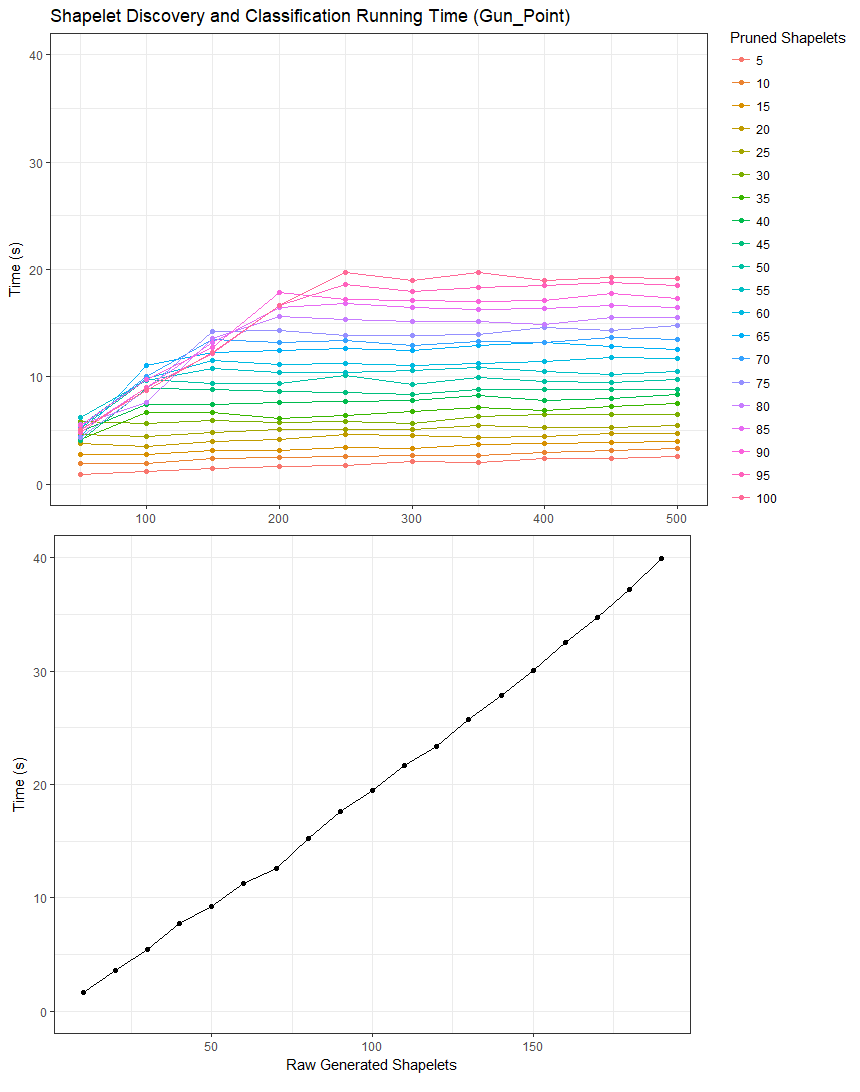
\includegraphics[width=0.8\textwidth]{Images/Time_comparison.png}
\caption{Plot of time taken for shapelet discovery and classification model training and testing. \textbf{Top}: Time taken using reduced SAX pruning methods. \textbf{Bottom}: Time taken using \textit{Ultra-Fast Shapelets} algorithm.}
\end{center}\end{figure}

\begin{figure}[ht]\begin{center}
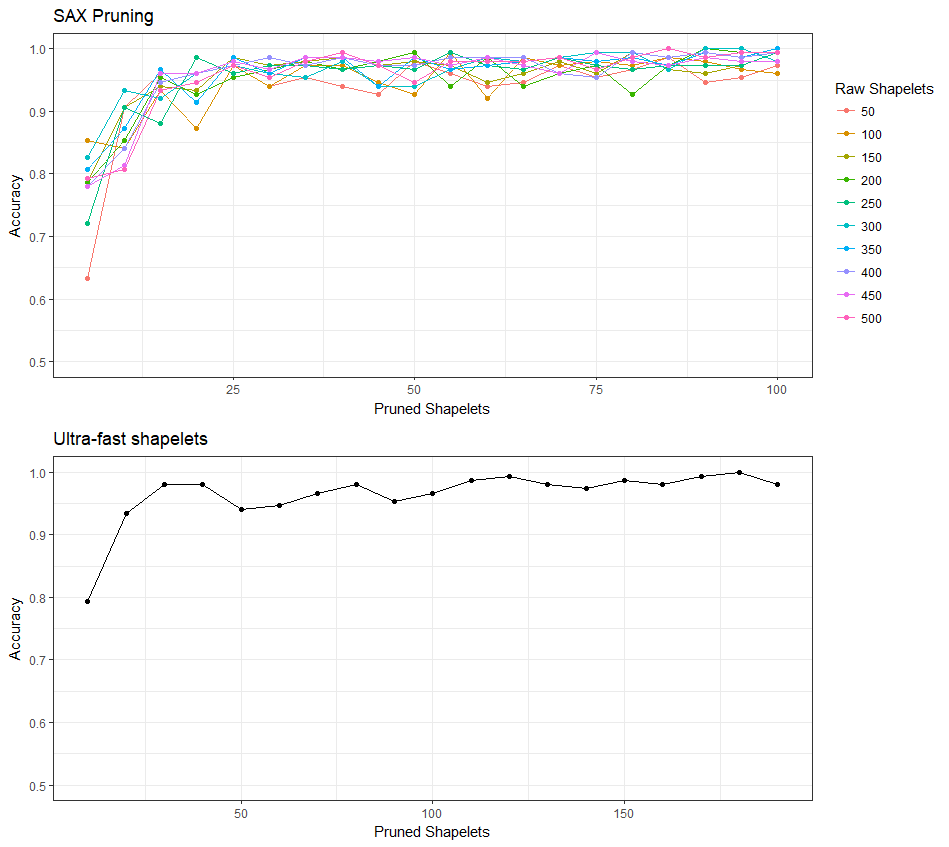
\includegraphics[width=0.8\textwidth]{Images/Accuracy_comparison.png}
\caption{Plot of accuracy of classification models created from shapelets discovered using two methods. \textbf{Top}: Accuracy using reduced SAX pruning methods. \textbf{Bottom}: Accuracy using \textit{Ultra-Fast Shapelets} algorithm.}
\end{center}\end{figure}


\section{Timeline}
\begin{tabular}{|l|c|c|c|c|c|c|c|c|c|c|c|c|}
\hline 
Week: & 1 & 2 & 3 & 4 & 5 & 6 & 7 & 8 & 9 & 10 & 11 & 12 \\ 
\hline 
Initial meeting & - & - & • &  &  &  &  &  &  &  &  &  \\ 
\hline 
Review of literature & - & - & • & • &  &  &  &  &  &  &  &  \\ 
\hline 
Writing proposal & - & - & • & • &  &  &  &  &  &  &  &  \\ 
\hline 
Replication of current research & - & - &  & • & • & • &  &  &  &  &  &  \\ 
\hline 
RSAX Development \& Testing & - & - &  &  &  & • & • & • &  &  &  &  \\ 
\hline 
Shapelet Scoring \& Pruning & - & - &  &  &  &  &  &  & • & • & • &  \\ 
\hline 
Project presentation & - & - &  &  &  &  &  &  &  &  &  & • \\ 
\hline 
Final report & - & - & • & • & • & • & • & • & • & • & • & • \\ 
\hline 
\end{tabular}

\pagebreak
\begin{thebibliography}{9}

\bibitem{1}
Rakthanmanon, T., \& Keogh, E. (2013, May). Fast shapelets: A scalable algorithm for discovering time series shapelets. In \textit{Proceedings of the 2013 SIAM International Conference on Data Mining} (pp. 668-676). \textit{Society for Industrial and Applied Mathematics}.
Retrieved from http://epubs.siam.org/doi/pdf/10.1137/1.9781611972832.74 

\bibitem{2}
Raza, A., \& Kramer, S. (2017). Ensembles of Randomized Time Series Shapelets Provide Improved Accuracy while Reducing Computational Costs. \textit{arXiv preprint arXiv}:1702.06712.

\bibitem{3}
Ye, L., \& Keogh, E. (2011). Time series shapelets: a novel technique that allows accurate, interpretable and fast classification. \textit{Data mining and knowledge discovery}, 22(1), 149-182.

\bibitem{4}
Shah, M., Grabocka, J., Schilling, N., Wistuba, M., \& Schmidt-Thieme, L. (2016, March). Learning DTW-shapelets for time-series classification. In \textit{Proceedings of the 3rd IKDD Conference on Data Science}, 2016 (p. 3). ACM.

\bibitem{5}
Petitjean, F., Forestier, G., Webb, G. I., Nicholson, A. E., Chen, Y., \& Keogh, E. (2016). Faster and more accurate classification of time series by exploiting a novel dynamic time warping averaging algorithm. \textit{Knowledge and Information Systems}, 47(1), 1-26.

\bibitem{6}
Lines, J., Davis, L. M., Hills, J., \& Bagnall, A. (2012, August). A shapelet transform for time series classification. In \textit{Proceedings of the 18th ACM SIGKDD international conference on Knowledge discovery and data mining} (pp. 289-297). ACM.\\
Available at \textbf{https://ueaeprints.uea.ac.uk/40201/1/LinesKDD2012.pdf}

\bibitem{7}
Wistuba, M., Grabocka, J., \& Schmidt-Thieme, L. (2015). Ultra-fast shapelets for time series classification. \textit{arXiv preprint} arXiv:1503.05018.

\bibitem{8}
Yanping Chen, Eamonn Keogh, Bing Hu, Nurjahan Begum, Anthony Bagnall, Abdullah
Mueen and Gustavo Batista (2015). The UCR Time Series Classification Archive. URL
$www.cs.ucr.edu/~eamonn/time_series_data/$

\end{thebibliography}

\end{document}
